\chapter{EFFECTIVE VISUALIZATIONS}
\label{effectiveVisualizationsChapter}
\section{Visual Information Seeking Mantra}
The visual information seeking mantra, defined by \cite{shneiderman1996eyes}, indicates that it is important to follow the steps overview first, zoom and filter, then details-on-demand when starting any information visualization. The dashboard was created with this in mind.
\subsection{Overview}
To achieve this aspect of the the dashboard starts by presenting all the data. An overview of the international food trade network, and particularly its complexity, can be seen immediately in the network graph (figure \ref{networkGraph}). The zoomed out view of both the network and cartographic maps allow for browsing the entirety of the collection.
\subsection{Zoom}
Zooming is done in both the cartographic and network visualizations. In the cartographic section it allows the user to see impacts to individual countries as in figure \ref{zoomed}. In the network graph section zooming facilitates exploration of geographically dense areas, such as Europe, (figure \ref{zoomedNetwork}).
	\begin{figure}[htb]
		\center{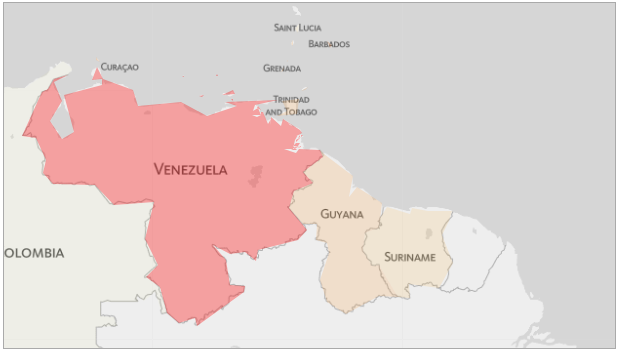
\includegraphics[width=\textwidth]{figures/zoomed.png}}
		\caption{A zoomed in view of the cartographic map.}
		\label{zoomed}
	\end{figure}
	\begin{figure}[htb]
		\center{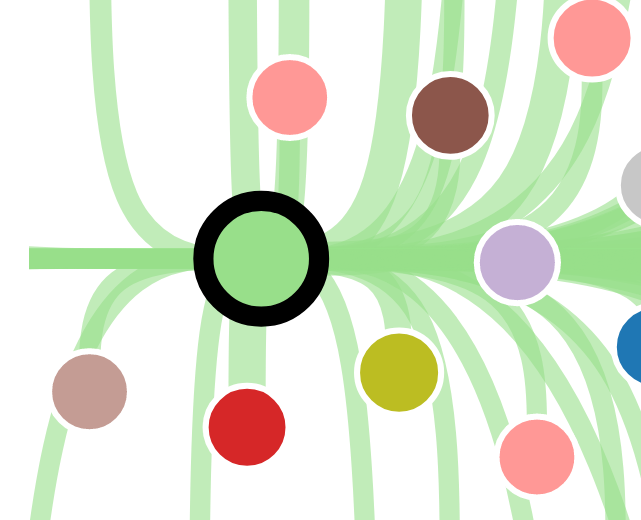
\includegraphics[width=\textwidth]{figures/zoomedNetwork.png}}
		\caption{A zoomed in view of the network graph.}
		\label{zoomedNetwork}
	\end{figure}
\subsection{Filter}
The tool allows filtering on a number of different parameters. The user can filter the trade good they wish to explore, the year they wish to examine, or the impacted country.
\subsection{Details on Demand}
Details are provided as tooltips in most sections of the dashboard. Hovering over the histograms show trade links that make up that particular bin. These can be used to identify susceptible trade links and prompt further filtering. A country's economic contribution in the network of the selected trade good can be seen by hovering over the country.
\section{Visual Analytics Dashboard}
\cite{keim2008visual} defines visual analytics as combining automated analysis techniques with interactive visualizations for an effective understanding, reasoning and decision making on the basis of very large and complex data sets.\par
The inclusion of prediction choropleth on the cartographic map helps transform the information visualization into a visual analytics tool. By aiding the user in making correlations we allow for that decision support. Allowing for filtering helps maintain the feedback loop \citep{keim2008visual} in which the user can make a decision.
